% !TEX root = ../thesis.tex
%
\chapter{Ablation Study}
In this chapter, we investigate the individual contributions of key factors influencing the performance and behavior of our proposed method.
Specifically, we focus on the effects of bias strength, the number of sensitive attributes, and the number of decisions on the system's overall functionality.
These factors are central to understanding the robustness and scalability of our approach.

\section{Bias Strength}
\label{sec:ablation_bias}
First, we will evaluate the sensitivity of the method to varying levels of inherent bias in the training data.
For this experiment, we used the \textit{cancer screening} model as a basis, due to its easily adjustable parameters.
While the model remains largely consistent with the version described in section \ref{sec:cancer_screening},
we modify the bias strength for the attribute \textit{gender} at the gateway following the activity \textit{assess screening eligibility},
which determines transitions to \textit{collect patient history} and \textit{refuse screening}.
Before, the probabilities to transition to either of these activities were split $0.7$ to $0.3$, depending on whether the patient is \textit{male} or \textit{female}.
In this analysis, we vary the probabilities to transition to \textit{collect patient history} for \textit{male} patients
and \textit{refuse screening} for \textit{female} patients,
incrementally from $0.5$ (perfectly equal) to $1.0$ (entirely biased) in steps of $0.05$.
The rest of the model remains identical.

For each step in bias strength and each of the three models (base, enriched and modified),
we perform 5-fold cross-validation and calculate the mean and standard deviation for both accuracy and demographic parity.
Analogously to the evalution of the \textit{cancer screening} model,
the demographic parity computation is performed by measuring the difference in selection rates between male and female patients for the \textit{collect history} transition,
using only samples where the previous event was \textit{assess eligibility}.
Therefore, when modifying the distilled decision tree, 
we remove each node that uses \textit{gender} as its splitting feature
and contains leaf nodes with the output classes \textit{collect patient history} and \textit{refuse screening} in its subtree.
The node removal is done via the retraining method.
The corresponding results are presented in Table \ref{tab:ablation_bias} and Figure \ref{fig:ablation_bias_accuracy}.

\begin{figure}[h!]
    \centering
    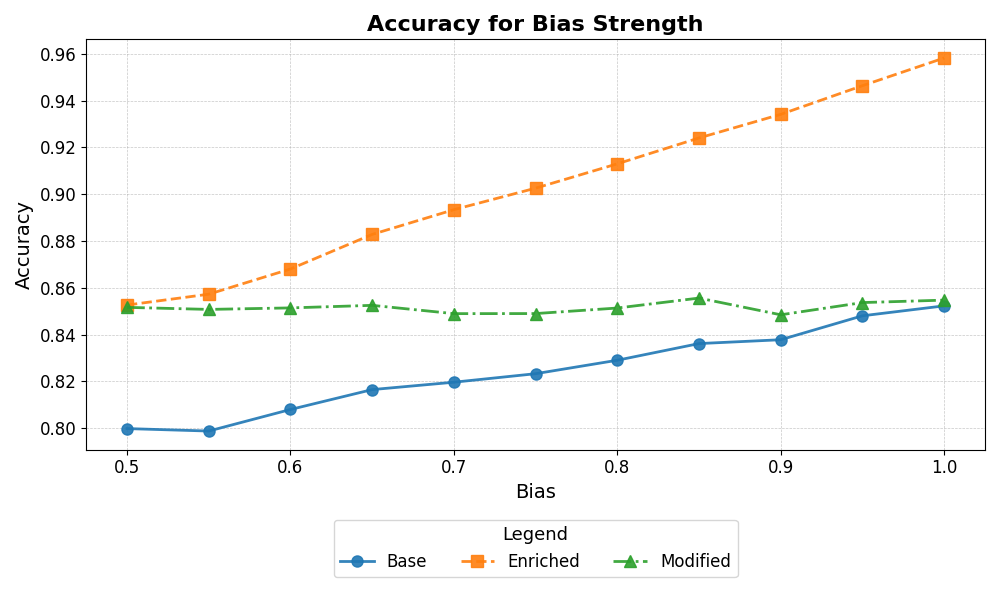
\includegraphics[width=0.9\textwidth]{gfx/ablation_bias_accuracy.png}
    \caption{Impact of varying bias strength on the accuracy.
    Each point in the graph represents the mean accuracy across validation folds for a certain bias strength.}
    \label{fig:ablation_bias_accuracy}
\end{figure}

\begin{table}[h!]
    \centering
    \scriptsize
    \renewcommand{\arraystretch}{1.2}
    \setlength{\tabcolsep}{6pt}
    \begin{tabularx}{\textwidth}{>{\centering\arraybackslash}m{1.7cm} | ccc | ccc}
        \toprule
        \textbf{Bias Strength} & \multicolumn{3}{c|}{\textbf{Accuracy}} & \multicolumn{3}{c}{\textbf{Demographic Parity}} \\
        & Base & Modified & Enriched & Base & Modified & Enriched \\
        \midrule
            0.50 &  .800 $\pm$ .001 &  .852 $\pm$ .002 &  .853 $\pm$ .003 &  .002 $\pm$ .001 &  .111 $\pm$ .222 &  .116 $\pm$ .231 \\
            0.55 &  .799 $\pm$ .005 &  .851 $\pm$ .003 &  .857 $\pm$ .006 &  .000 $\pm$ .000 &  .020 $\pm$ .035 &  .597 $\pm$ .487 \\
            0.60 &  .808 $\pm$ .003 &  .851 $\pm$ .002 &  .868 $\pm$ .004 &  .000 $\pm$ .001 &  .014 $\pm$ .022 &  .903 $\pm$ .183 \\
            0.65 &  .816 $\pm$ .002 &  .852 $\pm$ .002 &  .883 $\pm$ .003 &  .002 $\pm$ .001 &  .008 $\pm$ .014 &  .997 $\pm$ .002 \\
            0.70 &  .820 $\pm$ .003 &  .849 $\pm$ .003 &  .893 $\pm$ .002 &  .001 $\pm$ .001 &  .004 $\pm$ .006 &  .996 $\pm$ .002 \\
            0.75 &  .823 $\pm$ .003 &  .849 $\pm$ .003 &  .903 $\pm$ .002 &  .001 $\pm$ .002 &  .000 $\pm$ .000 &  .998 $\pm$ .002 \\
            0.80 &  .829 $\pm$ .004 &  .851 $\pm$ .002 &  .913 $\pm$ .003 &  .002 $\pm$ .002 &  .003 $\pm$ .001 &  .998 $\pm$ .001 \\
            0.85 &  .836 $\pm$ .002 &  .856 $\pm$ .003 &  .924 $\pm$ .001 &  .005 $\pm$ .003 &  .045 $\pm$ .038 &  .999 $\pm$ .000 \\
            0.90 &  .838 $\pm$ .005 &  .848 $\pm$ .004 &  .934 $\pm$ .002 &  .004 $\pm$ .003 &  .001 $\pm$ .000 &  1.00 $\pm$ .000 \\
            0.95 &  .848 $\pm$ .002 &  .854 $\pm$ .001 &  .946 $\pm$ .001 &  .006 $\pm$ .004 &  .003 $\pm$ .002 &  1.00 $\pm$ .001 \\
            1.00 &  .852 $\pm$ .003 &  .855 $\pm$ .002 &  .958 $\pm$ .001 &  .004 $\pm$ .002 &  .007 $\pm$ .008 &  1.00 $\pm$ .000 \\
        \bottomrule
    \end{tabularx}
    \vspace{0.2cm} % adds a small space between the two tables
    \caption{Evaluation of accuracy and demographic parity for varying bias strengths.
    The reported values represent the mean ($\mu$) and standard deviation ($\sigma$) across validation folds, expressed as $\mu \pm \sigma$.
    }

    \label{tab:ablation_bias}
\end{table}


\section{Number of Sensitive Attributes}  
Next, we will examine the behavior of our approach when varying the number of sensitive attributes for a single decision point.
For this purpose, we again use a modified version of the \textit{cancer screening} model described in section \ref{sec:cancer_screening}.
In this modified model, we remove the case attribute \textit{gender} and introduce $n$ generic categorical attributes $a_i$, with $i \in \{1, ..., n\}$.
Each of these attributes is considered to be sensitive and can take one of two possible values, $A$ or $B$, with a chance of 50\% each.

In a similar manner to the original \textit{gender} attribute, these attributes $a_i$ influence the same two decision gateways.  
However, since the transition probability at these gateways can no longer be determined directly by the value of a single attribute,
we follow an approach where each attribute contributes a weight that allows us to calculate the appropriate transition probabilities.
The probability of selecting a particular transition is computed by multiplying the individual attribute weights,
normalized by the sum of the multiplied weights for all possible transitions.

The unfair bias, which we aim to mitigate in the \textit{cancer screening} model, still occurs at the gateway after \textit{assess screening eligibility}.
The transition leading to \textit{collect patient history} is assigned a weight of $0.7$ by each generic attribute with the value $A$ and $0.3$ by each attribute with the value $B$.
Conversely, the transition leading to \textit{refuse screening} is given a weight of $0.3$ when the attribute value is $A$ and $0.7$ when it is $B$.
For example, if we consider three attributes $a_1, a_2, a_3$ with the attributes values $A, B, A$,
the product of weights would be $0.7 \times 0.3 \times 0.7 = 0.147$ for \textit{collect patient history},
and $0.3 \times 0.7 \times 0.3 = 0.063$ for \textit{refuse screening}.
Consequently, the resulting transition probabilities are $\frac{0.147}{0.147+0.063} = 0.7$ for \textit{collect patient history}
and $\frac{0.063}{0.147+0.063} = 0.3$ for \textit{refuse screening}.

The attributes $a_i$ also effect the gateway after \textit{collect patient history},
when deciding whether an individual should proceed to \textit{prostate screening} or \textit{mammary screening},
representing bias that we consider to be acceptable.
When assigning the corresponding weights for the possible transitions, we introduce a dependency on the index of the attribute.
If the index $i$ of an attribute $a_i$ is even, the transition to \textit{collect patient history} is assigned a weight of $0.7$
when the attribute takes the value $A$ and $0.3$ when it takes the value $B$,
while the transition to \textit{refuse screening} is given the weight of $0.3$ for $A$ and $0.7$ for $B$.
However, when the index $i$ is odd, these weight assigments are reversed for the values $A$ and $B$.
This is done to circumvent the effect observed in the previous ablation study from section \ref{sec:ablation_bias},
where an increased selection rate for \textit{collect patient history} automatically leads to an increased selection rate for \textit{prostate screening}.

We evaluate the model by varying the number of attributes up to 10 in increments of 2.
The demographic parity computation is performed by measuring the difference in selection rates between attribute values $A$ and $B$
for the \textit{collect history} transition, averaged over all attributes $a_i$,
using only samples where the previous event was \textit{assess eligibility}.
Similar to the ablation study for bias strength, when modifying the distilled decision tree,
we remove each node that uses an attribute $a_i$ as its splitting feature
and contains leaf nodes with the output classes \textit{collect patient history} and \textit{refuse screening} in its subtree.
Due to the high amount of potentially biasing attributes, 
utilizing the retraining method when removing nodes would likely introduce new unwanted biases in the retrained subtree,
requiring many iterations of retraining in an already long evaluation process.
Therefore, we applied the method of cutting branches instead.
Again, we employ 5-fold cross-validation for each increment and model.
The results are reported in Table \ref{tab:ablation_attributes} and Figure \ref{fig:ablation_attributes_accuracy}.


\begin{figure}[h!]
    \centering
    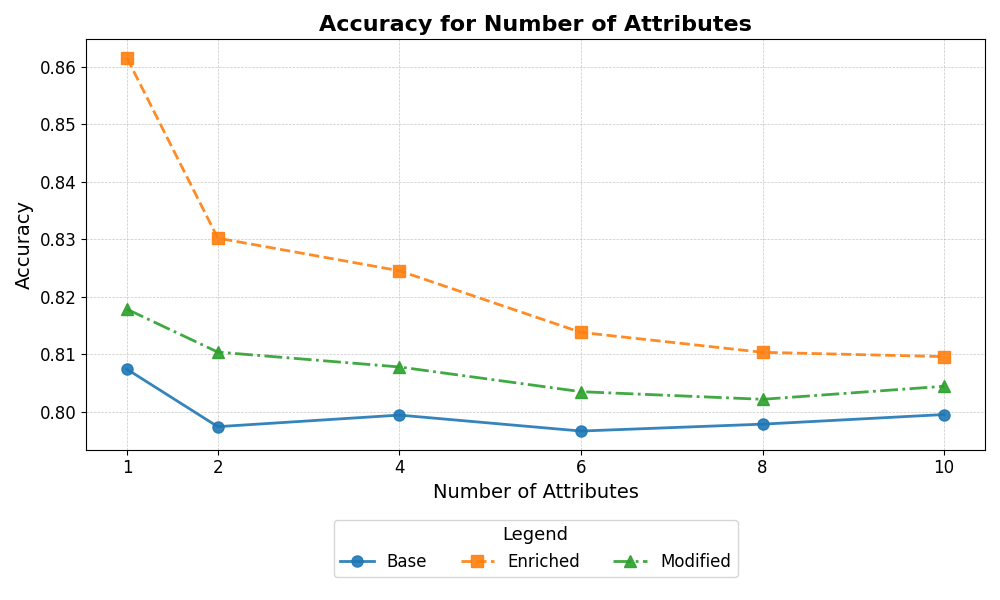
\includegraphics[width=0.9\textwidth]{gfx/ablation_attributes_accuracy.png}
    \caption{Impact of varying number of sensitive attributes on the accuracy.
    Each point in the graph represents the mean accuracy across validation folds for a certain number of attributes.}

    \label{fig:ablation_attributes_accuracy}
\end{figure}

\begin{table}[h!]
    \centering
    \scriptsize
    \renewcommand{\arraystretch}{1.2}
    \setlength{\tabcolsep}{6pt}
    \begin{tabularx}{\textwidth}{>{\centering\arraybackslash}m{1.7cm} | ccc | ccc}
        \toprule
        \makecell{\textbf{Num.} \\ \textbf{Attributes}} & \multicolumn{3}{c|}{\textbf{Accuracy}} & \multicolumn{3}{c}{\textbf{Demographic Parity}} \\
        & Base & Modified & Enriched & Base & Modified & Enriched \\
        \midrule
        1 &  .807 $\pm$ .003 &  .818 $\pm$ .003 &  .862 $\pm$ .005 &  .000 $\pm$ .000 &  .001 $\pm$ .000 &  .998 $\pm$ .000 \\
        2 &  .797 $\pm$ .005 &  .810 $\pm$ .004 &  .830 $\pm$ .003 &  .001 $\pm$ .001 &  .004 $\pm$ .001 &  .495 $\pm$ .067 \\
        4 &  .799 $\pm$ .003 &  .808 $\pm$ .005 &  .825 $\pm$ .004 &  .000 $\pm$ .000 &  .009 $\pm$ .000 &  .376 $\pm$ .038 \\
        6 &  .797 $\pm$ .003 &  .803 $\pm$ .007 &  .814 $\pm$ .006 &  .001 $\pm$ .000 &  .010 $\pm$ .004 &  .273 $\pm$ .027 \\
        8 &  .798 $\pm$ .003 &  .802 $\pm$ .002 &  .810 $\pm$ .005 &  .001 $\pm$ .000 &  .033 $\pm$ .014 &  .211 $\pm$ .039 \\
        10 &  .799 $\pm$ .003 &  .804 $\pm$ .002 &  .810 $\pm$ .003 &  .003 $\pm$ .002 &  .033 $\pm$ .010 &  .157 $\pm$ .051 \\
        \bottomrule
    \end{tabularx}
    \vspace{0.2cm} % adds a small space between the two tables
    \caption{Evaluation of accuracy and demographic parity for a varying amount of sensitive attributes.
    The reported values represent the mean ($\mu$) and standard deviation ($\sigma$) across validation folds, expressed as $\mu \pm \sigma$.
    }
    \label{tab:ablation_attributes}
\end{table}


\section{Number of biased Decisions}
In this section, we examine the effect of varying the number of decision points that utilize sensitive attributes in the model.
Similar to the previous ablation study on the number of sensitive attributes,
this study aims to assess the scalability of our method when multiple decisions in a process model introduce biased behavior. 

The models and event logs considered so far do not contain a sufficient number of meaningful decision points to conduct this analysis.
Therefore, we use a deliberately constructed process model that allows for a controlled evaluation of our approach.
This model consists of a \textit{start} activity and an \textit{end} activity.
Between these, it contains $n$ groups of four activities, denoted as $A_i$, $B_i$, $C_i$, and $D_i$, where $i \in \{1, ..., n\}$.
Each group represents a decision structure in which an incoming case must follow one of two possible paths, determined by a sensitive attribute. 
Similar to the previous experiment, we introduce $n$ sensitive categorical attributes $a_i$, where each $a_i$ takes the value $A$ or $B$ with an equal probability of 50\%.
Each attribute $a_i$ affects two decision gateways within its respective group.

The first decision occurs when entering the $i$-th group, where the transition probabilities are biased as follows:
If $a_i = A$, the probability of selecting $A_i$ is $0.7$, while the probability of selecting $B_i$ is $0.3$.
Conversely, if $a_i = B$, the probability of selecting $A_i$ is $0.3$, and the probability of selecting $B_i$ is $0.7$.
These decisions, concerning the events $A_i$ and $B_i$, introduce the unfair bias that we aim to remove in our model. 

The second decision occurs after $A_i$ or $B_i$, determining whether the process continues to $C_i$ or $D_i$.
This decision is structured in a similar way:
If $a_i = A$, the probability of selecting $C_i$ is $0.7$, while the probability of selecting $D_i$ is $0.3$.
If $a_i = B$, the probabilities are reversed, with $C_i$ receiving a probability of $0.3$ and $D_i$ a probability of $0.7$.
The biases in these decisions, concerning the events $C_i$ and $D_i$, are considered to be acceptable.
As such, our approach should retain these biases while mitigating the unfair bias at the first decision point in each group. 

\begin{figure}[h!]
    \centering
    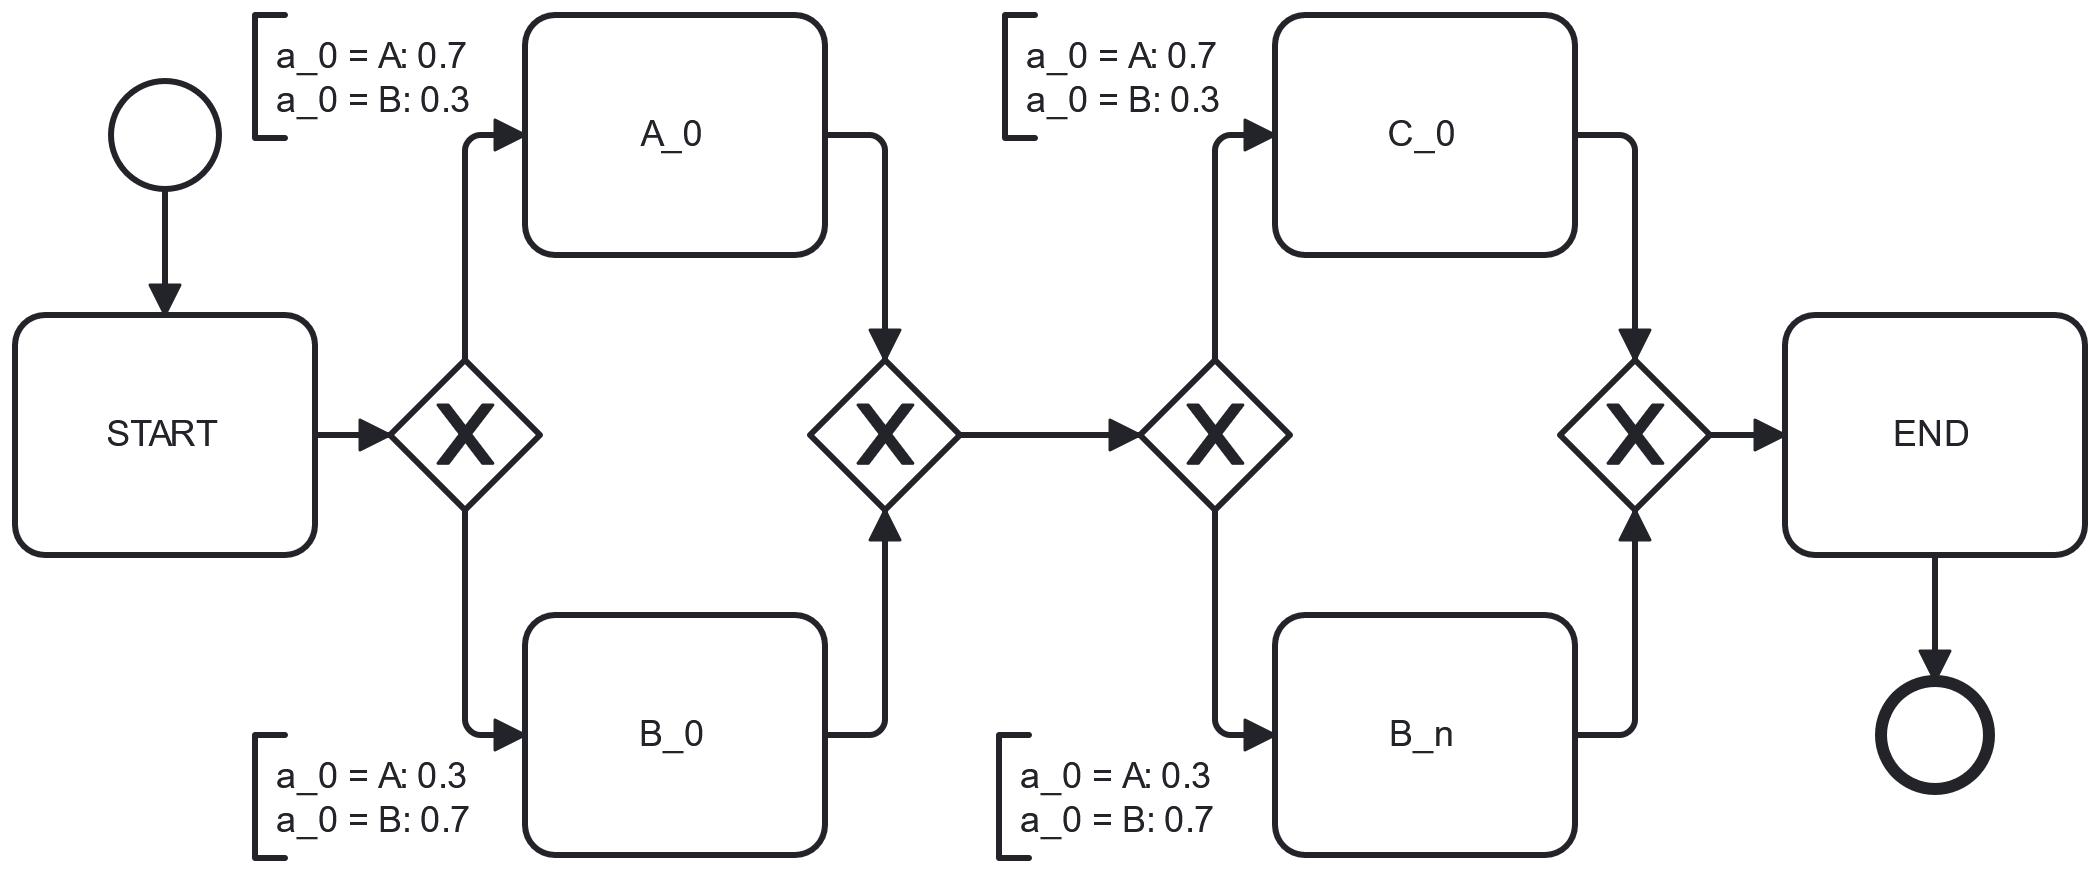
\includegraphics[width=\textwidth]{gfx/ablation_decision.png}
    \caption{The process model with only a single group consisting of the activities $A_0, B_0, C_0$ and $D_0$, influenced by the attribute $a_0$.
    Additional groups would be added between the last gateway, after activities $C_0$ and $D_0$, and the \textit{end} activity.}
    \label{fig:ablation_decision_model}
\end{figure}

Since each of the $n$ groups introduces two biased decision points, a model containing $n$ groups corresponds to a model with $2n$ biased decisions.
We inspect the number of biased decisions up to 20, in increments of 4. 
When mitigating the unfair bias in the distilled decision tree,
we remove each node that uses an attribute $a_i$ as its splitting feature and contains $A_i$ and $B_i$ as leaf nodes within its subtree.
As before, given the high number of biased decisions, applying the retraining method would introduce additional unwanted biases in the retrained subtree.
Therefore, we again use the method of cutting branches for node removal. 
The results from applying 5-fold cross-validation for each increment and model are reported in Table \ref{tab:ablation_decisions} and Figure \ref{fig:ablation_decisions_accuracy}. 

%TODO: correct text in image
\begin{figure}[h!]
    \centering
    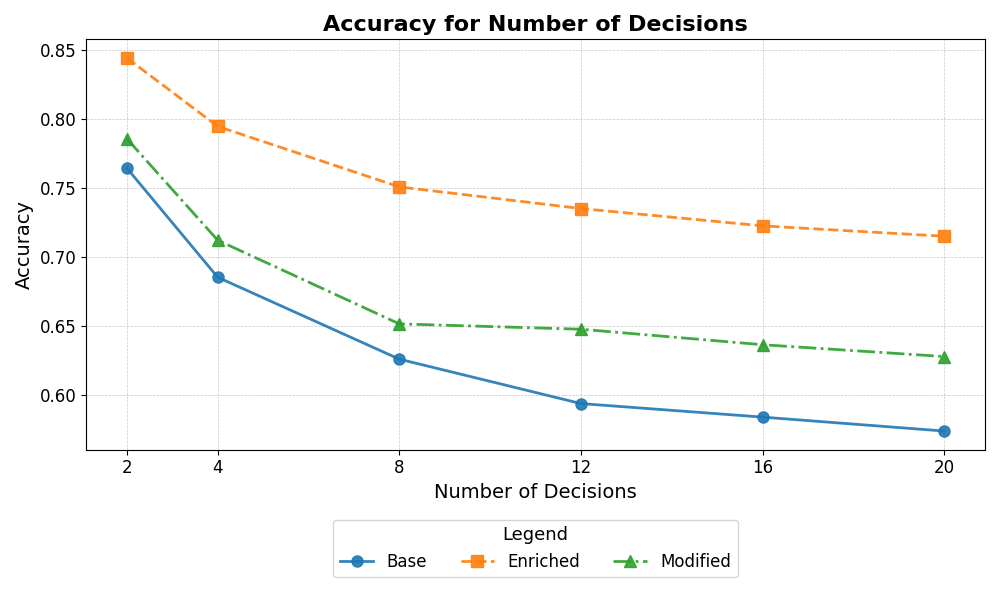
\includegraphics[width=0.9\textwidth]{gfx/ablation_decisions_accuracy.png}
    \caption{Impact of varying number of biased decisions on the accuracy.
    Each point in the graph represents the mean accuracy across validation folds for a certain number of decisions.}
    \label{fig:ablation_decisions_accuracy}
\end{figure}

\begin{table}[h!]
    \centering
    \scriptsize
    \renewcommand{\arraystretch}{1.2}
    \setlength{\tabcolsep}{6pt}
    \begin{tabularx}{\textwidth}{>{\centering\arraybackslash}m{1.7cm} | ccc | ccc}
        \toprule
        \makecell{\textbf{Num.} \\ \textbf{Decisions}} & \multicolumn{3}{c|}{\textbf{Accuracy}} & \multicolumn{3}{c}{\textbf{Demographic Parity}} \\
        & Base & Modified & Enriched & Base & Modified & Enriched \\
        \midrule
            2 &  .764 $\pm$ .003 &  .786 $\pm$ .017 &  .844 $\pm$ .004 &  .001 $\pm$ .000 &  .002 $\pm$ .000 &  .997 $\pm$ .000 \\
            4 &  .685 $\pm$ .005 &  .712 $\pm$ .018 &  .795 $\pm$ .002 &  .002 $\pm$ .002 &  .011 $\pm$ .008 &  .997 $\pm$ .003 \\
            8 &  .626 $\pm$ .002 &  .652 $\pm$ .015 &  .751 $\pm$ .002 &  .001 $\pm$ .001 &  .004 $\pm$ .003 &  .995 $\pm$ .002 \\
            12 &  .594 $\pm$ .004 &  .648 $\pm$ .002 &  .735 $\pm$ .001 &  .001 $\pm$ .001 &  .006 $\pm$ .006 &  .992 $\pm$ .008 \\
            16 &  .584 $\pm$ .002 &  .636 $\pm$ .002 &  .723 $\pm$ .001 &  .005 $\pm$ .005 &  .003 $\pm$ .004 &  .978 $\pm$ .014 \\
            R&  .574 $\pm$ .003 &  .628 $\pm$ .002 &  .715 $\pm$ .001 &  .004 $\pm$ .004 &  .002 $\pm$ .003 &  .977 $\pm$ .009 \\
        \bottomrule
    \end{tabularx}
    \vspace{0.2cm} % adds a small space between the two tables
    \caption{Evaluation of accuracy and demographic parity for a varying amount of biased decisions.
    The reported values represent the mean ($\mu$) and standard deviation ($\sigma$) across validation folds, expressed as $\mu \pm \sigma$.
    }
    \label{tab:ablation_decisions}
\end{table}

\section{Discussion}
% 